\documentclass [a4paper,11pt]{article}
\usepackage{uarial}
\usepackage[english]{babel}
\usepackage[toc,page]{appendix}

% Format the chapter headings
\usepackage[T1]{fontenc}
\usepackage{titlesec, blindtext, color}
\usepackage[hidelinks]{hyperref}

% Basic A4 paper settings with extra space
\usepackage[a4paper]{geometry}
\usepackage{a4wide}

% Input encoding as UTF8
\usepackage[utf8]{inputenc}

% For figures
\usepackage{graphicx}
\usepackage{caption}
\usepackage{subcaption}
\usepackage{wrapfig}
\usepackage{float}

% For math formulas
\usepackage{amsmath}
\usepackage{amssymb}
\usepackage{amsthm}

% For euro sign
\usepackage{eurosym}
%diametersign
\usepackage{wasysym}

% For lists
\usepackage{tabto}
\usepackage{enumitem}

\bibliographystyle{ieeetr}

% Title and authors
\title{Research Report}
\author{Jens Voortman \and Ruben Visser \and Vasco de Bruijn}

\newcommand{\rulesep}{\unskip\ \vrule\ }

\begin{document}

\begin{titlepage}

\newcommand{\HRule}{\rule{\linewidth}{0.5mm}}
\centering

\HRule \\[0.4cm]
{ \huge \bfseries Research Report}\\ % Title of your document
\HRule \\[0.4cm]

\textsc{\large Exoskeleton Monitoring System}\\[1.4cm]


\includegraphics[scale=0.1]{Project_MARCH2}\\[1.4cm]


\begin{minipage}{0.4\textwidth}
\begin{flushleft} \large
\emph{Authors:}\\
Jens Voortman\\
Ruben Visser\\
Vasco de Bruijn
\end{flushleft}
\end{minipage}
~
\begin{minipage}{0.4\textwidth}
\begin{flushright} \large

\includegraphics{logo_black}
\end{flushright}
\end{minipage}\\[2cm]

{\large \today}\\

\vfill
\end{titlepage}

% Create table of contents
\pagebreak
\tableofcontents
\pagebreak

% Final Chapter Order
% 1. Overview
% 2. Problem Definition & Analysis
% 3. Infrastructure
% 4. Development Methods
% 5. Design Goals
% 6. Requirements
% 7. Data Transfer
% 8. Data Analysis
% 9. User Interface

\section{Problem definition \& analysis}
\subsection{Problem definition}
In 2015, the ``Moving Bird Foundation'' was founded. As part of the foundation, the dream team ``Project MARCH'' was created. The goal of this dream team is designing and building an exoskeleton for paraplegic people, to participate in the `Powered Exoskeleton Race'-discipline of the 2016 Cybathlon in Zurich\footnote{\url{http://www.cybathlon.ethz.ch/en/}}. The Cybathlon is the first `Olympics' for disabled athletes using bionic assistive technology.\\ 
The exoskeleton that is being designed has many sensors, which acquire data from their surroundings. Project MARCH wishes to have a system, which allows for external monitoring and visualization of all vital sensor data.

\subsection{Problem Analysis}
During this project the team is tasked to design and implement an external system, that hooks into the existing system and makes the monitoring of the sensors possible. Currently there is no wireless connection, the only way to check the sensor data is by connecting the exoskeleton to an external PC with a LAN-cable. This way of connecting is not preferred, as it has the possibility to impede the movement of the exoskeleton.\\ Furthermore, as it stands now only the raw sensor data can be extracted, which is of no use since this data is unitless. It's important to be able to monitor the sensors in a comprehensible way, as the MARCH-team will be able to stop the exoskeleton sooner if anything happens to be failing.
\pagebreak
\section{Existing Infrastructure}
\subsection{EtherCat}

\subsection{Output Sensors}
In order to monitor MARCH, it contains several sensors. Each sensor corresponds with a certain part of the exoskeleton and a certain type of measurement. The joints of MARCH that require monitoring are the hip joints, the knee joints and the ankle joints . MARCH contains  types of sensors:
\subsubsection{IMU}
An inertial measurement unit (IMU) is a device that measures and reports a craft's velocity, orientation, and gravitational forces. Each joint of MARCH contains an IMU. Together those IMU's are used to keep track of the position as well as the movement of the legs. The IMU's are also used to calculate the center of mass. 
\subsubsection{Proximity sensors}
Proximity sensors are devices used to measure the distance based on the speed of light/sound. The eight proximity sensors are situated on the feet and are for range feedback. They are situated as such: two at the bottom (front and back of the foot) and the other two on the edges towards the anterior and posterior coronal plane on the soles of the feet (again front and back). 

\subsubsection{Encoders}
An encoder is a device that measures angular position or motion of a shaft or axle. MARCH contains in total 12+4 Rotary Encoders in all of the joints and +6 in each motor. Each joint has one Torque and one Angle encoder, while each Foot-Joint contains 2 more for the Ankle-AFE and AAA. Each motor has only a Torque encoder.
\subsubsection{Range Finders}
The six range finders are situated on the two shanks and are for range feedback. They work by using echolocation.
\subsubsection{Force/torque sensors}
The four force/torque sensors are situated on the bottom of the feet.

\subsection{Simulink}
\pagebreak
\section{Development Methodology}
\pagebreak
\section{Requirements}\label{sec:req}
From the problem definition and analysis, we composed a list of requirements.
After meeting with the Client Advisor to discuss this list, the following table was the result and will be taken in consideration in the rest of the report:\\

{\renewcommand{\arraystretch}{1.5}
	\centering
	\begin{tabular}{ | l | l | }
		\hline
		\bfseries{Priority} & \bfseries{Requirement} \\ \hline
		M & Establish a wireless connection \\ \hline
		M & Send sensor data over a wireless connection \\ \hline
		M & Format data in a comprehensible way \\ \hline
		M & Access sensor data by CLI on external PC \\ \hline
		M & Work with custom Simulink block (API) \\ \hline
		S & Basic GUI for sensor data on external PC \\ \hline
		C & Sophisticated GUI for sensor data on external PC\\ \hline
		C & Graphical representation of sensor data in GUI\\ \hline
		C & Data logging on the external system \\ \hline
		W & Represent the exoskeleton with a 3D-model in the GUI based on the data \\ \hline
		W & Broadcast analysed data to multiple interfaces \\ \hline 
		W & Send commands from external system to exoskeleton \\ \hline 
	\end{tabular}
	\captionof{table}{Priorities ordered with the MoSCoW method} 
	\label{table:requi}
}
\pagebreak
\section{Wireless Data Transfer}
This section describes the most important point for the research. If the data is not transferred wireless to the external system blablabla

\subsection{Original idea}
EtherCAT is already used on the exoskeleton as stated in section \ref{sec:etherCat}. This lead to the first point, whether the current EtherCAT-configuration could be extended. The exoskeleton (E) and the receiver (R) would both be running Simulink. The receiver would then process the data and send it to the interface (I). This leaves the possibility to  extend to multiple interfaces, by putting a broadcaster (B) between the receiver and the interface(s). A visual representation of this model can be found in figure \ref{fig:catmodel}. However, the EtherCAT-blocks in Matlab \cite{web:ethercat} do not support wireless connections. Therefore it is not possible to implement this solution.

The next step was to check whether the original model would work using the Ethernet-blocks \cite{web:ethernet} instead. The original model would only need a slight change, which results in figure \ref{fig:netmodel}. However, after consulting with Speedgoat, this model was deemed as not preferred. If a USB wireless adapter would be used, drivers would need to be written for it as Simulink cannot use the standard drivers.\\
Timeframe en tijd enzo\\

\begin{figure}[H]
	\centering
	\begin{minipage}{.49\textwidth}
		\centering
		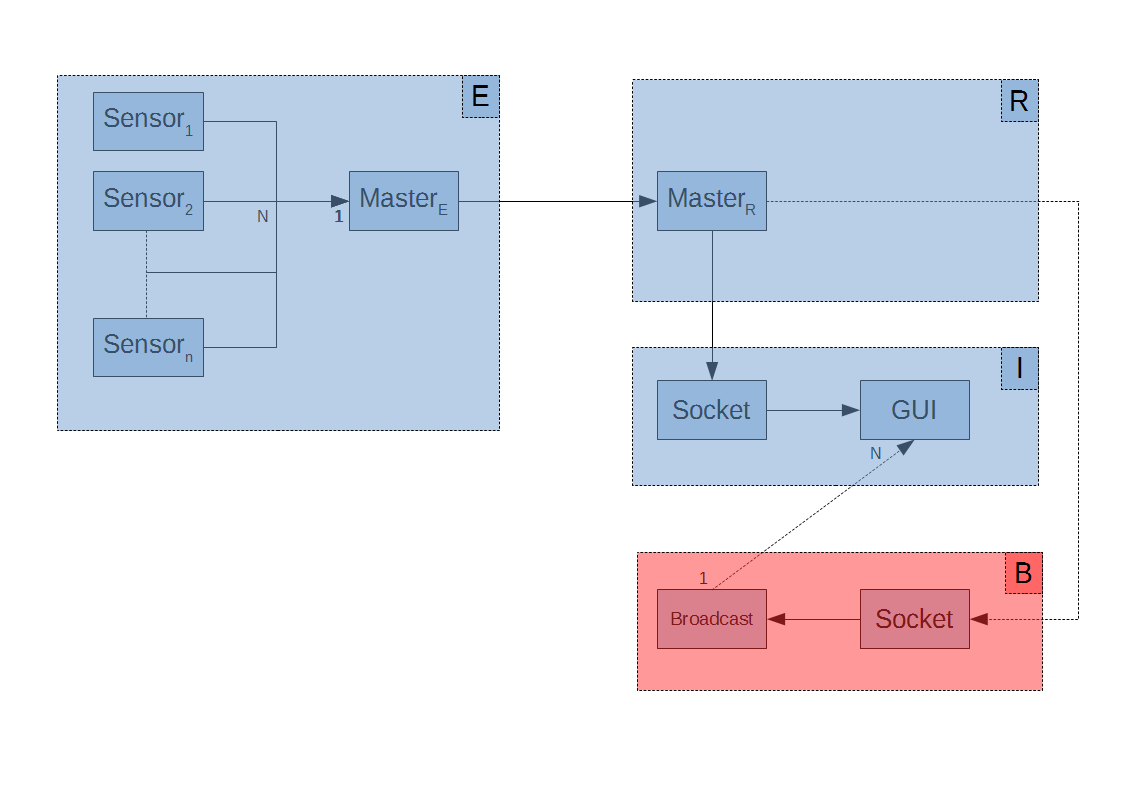
\includegraphics[width=\linewidth]{ERBI-Model-EtherCat}
		\subcaption{EtherCAT variation}
		\label{fig:catmodel}
	\end{minipage}
	\rulesep
	\begin{minipage}{.49\textwidth}
		\centering
		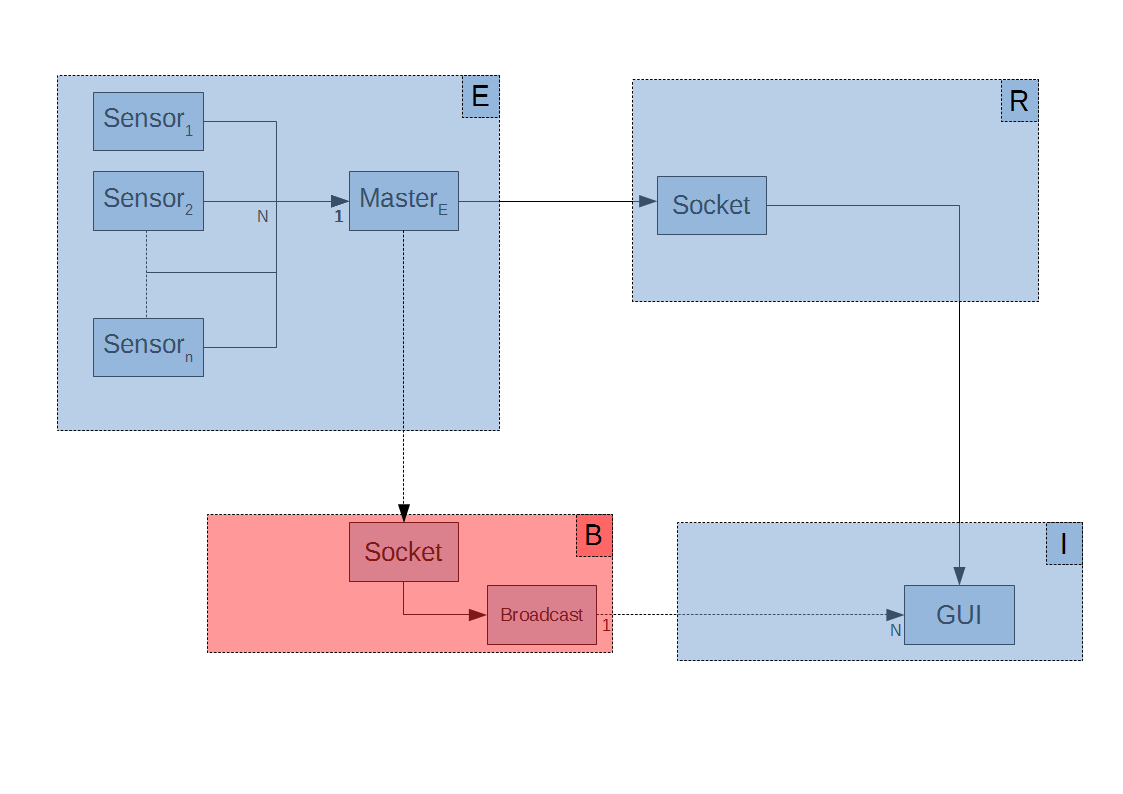
\includegraphics[width=\linewidth]{ERBI-Model-TCP}
		\subcaption{Ethernet variation}
		\label{fig:netmodel}
	\end{minipage}
	\caption{The variations of the original model}
	\label{fig:firstmodel}
\end{figure}

\subsection{Improved models}
Due to a lack of options to add wireless communication directly to the Speedgoat, bridging hardware is required to attach a wireless card on a wired interface on the Speedgoat. The following models are based on the possibility to build a wireless connection via such a device. 
\subsubsection{Plan A1}
This model requires the wireless bridge to transparently bridge the wired and wireless connections on the network level. This makes direct communication between the data provider (E) and client (I) possible. The Simulink model on the exoskeleton can directly send acquired data to a client with a GUI build in Matlab. By using Matlab to build the GUI we can make use of the extensive data visualization features and data processing features of Matlab without the need of translating this data for use with another program. 

Although the chosen networking model does not differentiate between networking protocols, UDP send \cite{web:UDPSend} is considered as a good choice due to the ease of setting up non-blocking communication.
% En nog iets met UDPSend! UDP Send: \cite{web:UDPSend}
\subsubsection{Plan A2}
Also this solution comprises of a data provider in Simulink running on the exoskeleton and a Matlab client, however the networking model is slightly different. Instead of building a transparent connection bridge, the wireless bridge will run software listening for connections both on the wireless and wired network connection. This will eliminate the need to use server sockets on the exoskeleton and on the client, instead both of them will build a connection to the bridge. The software running on the bridge will ensure that data pushed from the exoskeleton will be pushed further to any connected client.
\subsubsection{Plan B}
The Standalone Model with a non-Matlab executable running on the client can make use of the same two networking models. However, if the solution similar to Plan A2 is chosen, the bridge might be used too as a data processing unit. The advantage of this is that the data can be transformed to a format that eases the processing on the client.
\subsubsection{Plan C}
The Webservice Model avoids the need of running a standalone executable or the need of a Matlab installation on the system running the client. The client connects to the network, and the full interface can be opened in a web browser by pointing the location to the url of the bridge. This will require data processing on the bridge, as it has to reformat the data send by simulink on the exoskeleton to a format suitable for sending over a websocket to the client. The client can not use a technique like polling because of the need for real-time data.

\subsection{Data Packaging}
\begin{itemize}
	\item Two custom blocks in Matlab
	\item State Table
	\item Update rate 50 Hz
\end{itemize}
\pagebreak
\section{Data Processing}\label{sec:dataproc}
\subsection{Data Packaging}
\begin{itemize}
	\item Two custom blocks in Matlab
	\item State Table
	\item Update rate 50 Hz
\end{itemize}
\subsection{Converting Raw Data}
%TODO Correcte weergave data vs snel weergave data

\pagebreak
\section{User Interface}
\subsection{Description}
When the sensor data has arrived at the remote PC, the data has to be read out. The data should be at least be output to a console. If possible due to time constraints, the data will be more visualised.
\subsubsection{CUI}
The CUI (Console User Interface) is the most basic way the data will be output. All the sensor data will be output to the control with corresponding label. The CUI will automatically be updated when new data arrives. 
\begin{figure}[H]
	\centering
	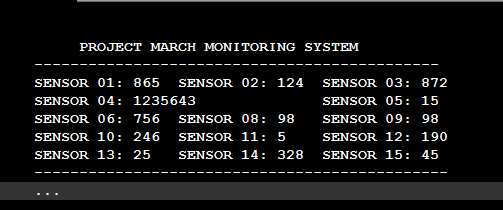
\includegraphics[width=.75\textwidth]{MockupCUI}
	\caption{A mock-up with a possible look of the CUI} 
\end{figure} 
\subsubsection{GUI}
The GUI (Graphic User Interface) consists of two parts. One part shows a dashboard with the most important sensor data visualised. The other part is a concise list with all sensor data.  
\begin{figure}[H]
	\centering
	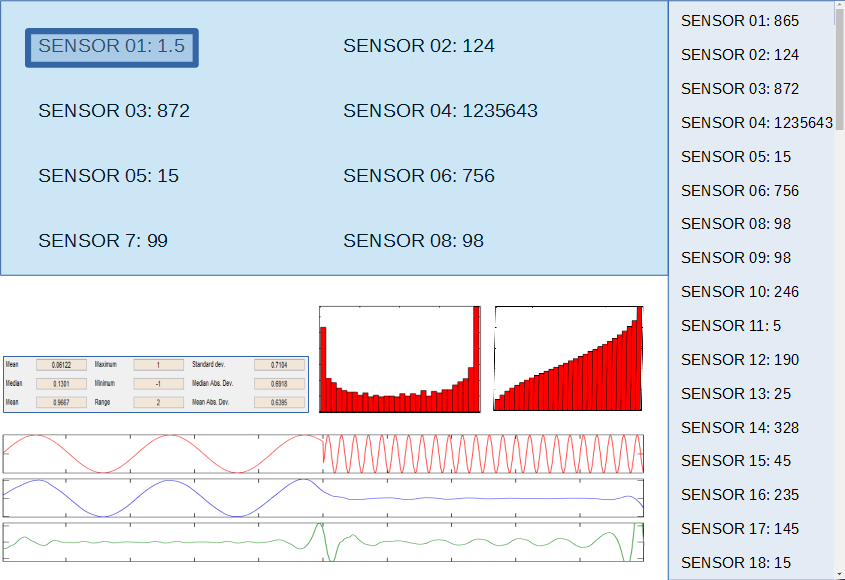
\includegraphics[width=.75\textwidth]{MockupGUI}
	\caption{A mock-up with a possible look of the GUI} 
\end{figure} 
\subsection{Languages}
For this project, it is important to use a language which has rich support for data visualisation and 3d-rendering. In addition, the chosen language must be able to (easily) interface Matlab since the sensor data will enter via a SimuLink model. In addition to the MATLAB language, C/C++, Java \& Python are valid options since Matlab has a build-in interface for these languages and these languages have libraries which support 3D rendering and data visualisation.\\ 


The requirements state that data visualisation has a higher priority than 3D-rendering. Because of this, it is not essential that the chosen framework has an extensive 3D-library. In the end, Matlab was chosen as preferred framework for the GUI for the following reasons:
\begin{itemize}
	\item The required data is sent through SimuLink, which is a module of Matlab. This means that the data does not need to be converted.
	\item Matlab has an extensive collection of data visualisation tools.
	\item Most other applications within Project MARCH also make use of Matlab. Therefore, using Matlab helps future integration and easier continuation.
\end{itemize}
In the event that it proves to be impossible or undesirable to connect wireless directly using Matlab, there are three alternatives to consider. The first one is to create a receiver which listens on the port and can convert the data to a format which is readable by Matlab.
\\The second option would be to use a stand-alone application which is based on another framework than Matlab. This would widen the range of possibilities for the use of the interface.
\\The last option is to create the GUI in HTML as a web-page and put a web-socket in the page to get the data. This implementation is very user friendly, as the only required software for the client is a web-browser. In addition, this makes it very easy for multiple people to use the monitoring system since the exoskeleton will broadcast over the wi-fi instead of sending the data directly to another client. By using this method, the options for the framework are limited to JavaScript and its libraries. In addition, running code in a browser tends to be less powerful than running the code in a stand-alone application. This results in a lower update frequency and fewer options for data visualising.

\subsection{3D-Rendering}
Because of the fact that the 3d-rendering has shifted to a lower priority, less effort has been expended in researching suitable frameworks for rendering. Still, a small list have been compiled of some rendering frameworks which are simple to use for each of the narrowed down languages. In addition, Matlab also contains modules for 3d-rendering.
\begin{itemize}
	\item C/C++: Ogre3D \cite{web:ogre3d}
	\item Java/Scala: Env3D \cite{web:env3d}
	\item Python: Panda3D \cite{web:panda3d}
\end{itemize}
	
\pagebreak

\appendix
\bibliography{biblio}

\end{document}
